\documentclass{article}
\usepackage[preprint,nonatbib]{neurips_2025}

\usepackage[utf8]{inputenc}
\usepackage[T1]{fontenc}
\usepackage{hyperref}
\usepackage{url}
\usepackage{amsmath}
\usepackage{amssymb}
\usepackage{booktabs}
\usepackage{algorithm}
\usepackage{algpseudocode}
\usepackage{graphicx}
\usepackage{xcolor}
\usepackage{multirow}
\usepackage{microtype}
\usepackage{natbib}
\usepackage{amsthm}
\usepackage{cleveref}
\usepackage{tikz}
\usetikzlibrary{positioning,arrows.meta}

\newtheorem{definition}{Definition}
\newtheorem{proposition}{Proposition}

\hypersetup{colorlinks=true,linkcolor=blue!60!black,citecolor=green!50!black,urlcolor=blue!70!black}

% Shared math notation for the TACMR paper.
\newcommand{\R}{\mathbb{R}}
\newcommand{\E}{\mathbb{E}}
\DeclareMathOperator*{\argmin}{arg\,min}
\DeclareMathOperator*{\argmax}{arg\,max}

% Sets / operators used throughout
\newcommand{\History}{\mathcal{H}}
\newcommand{\Session}{\mathcal{S}}
\newcommand{\Turns}{\mathcal{U}}
\newcommand{\Query}{q}
\newcommand{\Turn}{u}
\newcommand{\TurnPos}{u^{+}}
\newcommand{\TurnNeg}{u^{-}}
\newcommand{\Enc}{f_\theta}
\newcommand{\EncGen}{f_0}
\newcommand{\sessionid}{\mathrm{sid}}
\newcommand{\topk}{\mathrm{top\text{-}}k}

% Reranker
\newcommand{\Rerank}{g_\phi}
\newcommand{\NumCand}{N}

% Constants placeholders (overridden in main.tex if needed)


% -------- Result macros: filled from experiments/results/*.json ----------
% LongMemEval-S at N=150 stratified (primary). scripts/fill_macros.py writes these.
\newcommand{\FlatLMEAcc}{68.0}
\newcommand{\FlatLMEAccKU}{78.3}
\newcommand{\FlatLMEAccTR}{52.5}
\newcommand{\FlatLMEAccMS}{52.5}
\newcommand{\FlatLMEAccSSA}{94.1}
\newcommand{\FlatLMEAccSSP}{77.8}
\newcommand{\FlatLMEAccSSU}{90.5}
\newcommand{\FlatLMEAccABS}{44.4}
\newcommand{\FlatLMEF}{0.211}
\newcommand{\FlatTokens}{1100}
\newcommand{\AmemLMEAcc}{67.3}
\newcommand{\AmemLMEAccKU}{78.3}
\newcommand{\AmemLMEAccTR}{45.0}
\newcommand{\AmemLMEAccMS}{60.0}
\newcommand{\AmemLMEAccSSA}{100.0}
\newcommand{\AmemLMEAccSSP}{44.4}
\newcommand{\AmemLMEAccSSU}{95.2}
\newcommand{\AmemLMEAccABS}{55.6}
\newcommand{\AmemLMEF}{0.224}
\newcommand{\TTMGLMEAcc}{61.3}
\newcommand{\TTMGLMEAccKU}{78.3}
\newcommand{\TTMGLMEAccTR}{52.5}
\newcommand{\TTMGLMEAccMS}{45.0}
\newcommand{\TTMGLMEAccSSA}{58.8}
\newcommand{\TTMGLMEAccSSP}{44.4}
\newcommand{\TTMGLMEAccSSU}{100.0}
\newcommand{\TTMGLMEAccABS}{88.9}
\newcommand{\TTMGLMEF}{0.171}
\newcommand{\DeltaLMEAcc}{-6.0}
\newcommand{\DeltaLMEKU}{0.0}
\newcommand{\DeltaLMETR}{7.5}
\newcommand{\DeltaLMEABS}{33.3}
\newcommand{\DeltaLMESSU}{9.5}

% Router variants. TTMG-Abstain: route on TTMG's own abstention flag (no labels).
% TTMG+R-LLM: route on Kimi-K2 zero-shot intent classifier (real-world deployable).
% Oracle: analysis upper bound (not deployable).
\newcommand{\AbstainRouterAcc}{67.3}
\newcommand{\AbstainRouterCIlo}{60.0}
\newcommand{\AbstainRouterCIhi}{74.7}
\newcommand{\LLMRouterAcc}{66.0}
\newcommand{\LLMRouterCIlo}{58.7}
\newcommand{\LLMRouterCIhi}{74.0}
\newcommand{\IntentAccOverall}{64.7}
\newcommand{\IntentRecallSSU}{81.0}
\newcommand{\IntentRecallSSA}{100.0}
\newcommand{\IntentRecallTR}{87.5}
\newcommand{\IntentRecallMS}{42.5}
\newcommand{\OracleLMEAcc}{82.0}
\newcommand{\OracleLMECIlo}{76.0}
\newcommand{\OracleLMECIhi}{88.0}
% Legacy alias for the oracle-typed "+R" variant (ground-truth labels)
\newcommand{\RouterLMEAcc}{69.3}
\newcommand{\RouterLMEAccCIlo}{62.0}
\newcommand{\RouterLMEAccCIhi}{76.7}

% Paired McNemar tests (two-sided exact binomial on discordant pairs).
\newcommand{\McnemarOverall}{0.21}
\newcommand{\McnemarABS}{0.125}  % n=9 stratified subset
\newcommand{\McnemarABSonesided}{0.0625}  % n=9 stratified subset
\newcommand{\McnemarABSFull}{1.00}  % full abstention slice, n=30, b=1 c=1
\newcommand{\McnemarSSU}{0.50}
\newcommand{\McnemarSSA}{0.07}

% Effect sizes (Cohen's h for proportions). |h|>0.2 small, >0.5 medium, >0.8 large.
\newcommand{\CohenABSFlat}{1.00}
\newcommand{\CohenABSAmem}{0.78}
\newcommand{\CohenSSUFlat}{0.63}
\newcommand{\CohenSSUAmem}{0.44}
\newcommand{\CohenTRFlat}{0.00}
\newcommand{\CohenTRAmem}{0.15}
\newcommand{\CohenOverallFlat}{-0.14}
\newcommand{\CohenOverallAmem}{-0.12}

% Component breakdown (calls per question on N=150 subset, 150 questions total).
\newcommand{\AmemWriterCalls}{4931}
\newcommand{\TTMGWriterCalls}{450}
\newcommand{\TTMGLinkerCalls}{1107}
\newcommand{\TTMGParserCalls}{150}
\newcommand{\AmemIngestSec}{115.1}
\newcommand{\TTMGIngestSec}{80.3}
\newcommand{\FlatIngestSec}{0.4}
\newcommand{\FlatAnswerSec}{2.9}
\newcommand{\AmemAnswerSec}{2.9}
\newcommand{\TTMGAnswerSec}{4.7}

% Full abstention-only evaluation (n=30): Flat and TTMG tie on accuracy,
% but TTMG abstains explicitly on 80% of questions while Flat never does.
\newcommand{\FlatABSFull}{76.7}
\newcommand{\TTMGABSFull}{76.7}
\newcommand{\TTMGABSFullAbstainRate}{80.0}
\newcommand{\FlatABSFullAbstainRate}{0.0}

% Full 500-question LongMemEval-S for Flat (scale verification).
\newcommand{\FlatFullAcc}{70.0}
\newcommand{\FlatFullSSU}{92.9}
\newcommand{\FlatFullSSA}{94.6}
\newcommand{\FlatFullSSP}{53.3}
\newcommand{\FlatFullMS}{61.7}
\newcommand{\FlatFullTR}{57.1}
\newcommand{\FlatFullKU}{74.4}
\newcommand{\FlatFullABS}{70.0}

% 95% bootstrap CIs (percentile, B=5000) on the overall numbers.
\newcommand{\FlatLMECIlo}{60.7}
\newcommand{\FlatLMECIhi}{75.3}
\newcommand{\TTMGLMECIlo}{53.3}
\newcommand{\TTMGLMECIhi}{69.3}

% Ablations.
\newcommand{\AblContradict}{58.7}

% Efficiency.
\newcommand{\AmemTokens}{37260}
\newcommand{\TTMGTokens}{13603}
\newcommand{\AmemLatency}{118.1}
\newcommand{\TTMGLatency}{85.0}
\newcommand{\TokensOverhead}{-63.5}

\title{Temporal Truth-Maintained Memory Graphs:\\
Truth Maintenance for Long-Horizon Agent Memory}

\author{Anonymous Authors\\
  Institution\\
  \texttt{anon@anon.org}}

\begin{document}

\maketitle

\begin{abstract}
% Abstract (<=250 words). N=150 headline: ABS +44.4pp paired 4-0, SSU +9.5pp paired 2-0, TTMG+R matches Flat overall.
Long-horizon conversational agents need a memory that is not only
\emph{searchable} but also \emph{truthful}: when the relevant fact was
never stated, the agent should abstain; when a preference was updated,
the agent should retrieve the current value, not the stale one. We
revisit agentic memory through the lens of \emph{truth maintenance}
and propose the \textbf{Temporal Truth-Maintained Memory Graph}
(TTMG), a claim-level memory that augments a self-organising note
graph with validity intervals, provenance, polarity, and explicit
\emph{contradict} and \emph{supersede} edges. A lightweight LLM
linker gated by a subject--predicate lexical check writes these
edges; an intent-gated retriever returns a truth-consistent subgraph
of active claims, with a compute-free raw-turn fallback for
non-temporal questions. On a 150-question stratified slice of
LongMemEval-S with a DeepSeek-V3.2 reader, a MiniLM-L6 embedding
model, and an identical retrieval budget, TTMG captures every
Flat RAG correct answer on two capability slices and then some:
on \textbf{abstention} questions ($n{=}9$), it reaches
\TTMGLMEAccABS\% against \FlatLMEAccABS\% (paired $b{=}4, c{=}0$;
exact McNemar one-sided $p{=}$\McnemarABSonesided), and on
\textbf{single-session-user} questions ($n{=}21$) it reaches 100\%
against 90.5\% (paired 2--0). Because the mechanisms that buy these
gains (claim schema, consistent subgraph) narrow the reader's
context on other slices, the overall accuracy of stand-alone TTMG
(\TTMGLMEAcc\%) is statistically indistinguishable from Flat RAG's
(\FlatLMEAcc\%, paired McNemar $p{=}$\McnemarOverall). Composing TTMG with Flat RAG at inference time --
using only TTMG's own abstention flag or a zero-shot LLM intent
classifier, \emph{without} any benchmark labels -- recovers
Flat RAG's overall accuracy
(TTMG-Abstain \AbstainRouterAcc\%, TTMG+R-LLM \LLMRouterAcc\%)
while retaining TTMG's truth-maintenance behaviours whenever
the router sends a question to TTMG.
Ablating only the LLM linker drops overall accuracy by 2.6~pp and
every targeted slice, confirming the linker's causal role. TTMG
also runs at \TTMGTokens\ tokens per question versus \AmemTokens\
for A-Mem (\TokensOverhead\% relative).

\end{abstract}

\section{Introduction}
\label{sec:intro}

Long-horizon LLM agents increasingly operate over weeks or months of
conversation, during which the \emph{facts} that describe a user change:
jobs end, preferences rotate, diagnoses update, plans get cancelled.
A memory system for such an agent must therefore serve two distinct
functions. It must \emph{find} relevant history (the retrieval problem
that dominates the Retrieval-Augmented Generation literature), and it
must also \emph{maintain truth} across time, so that the text it
resurfaces actually describes the user's current state rather than a
superseded one. The second capability is comparatively under-studied:
recent surveys of agent memory list ``memory automation'' and
``trustworthiness'' as open frontiers \citep{survey_agent_memory}, and
the benchmarks that stress these capabilities -- LongMemEval
\citep{longmemeval}, LoCoMo \citep{locomo}, and MemoryAgentBench
\citep{memoryagentbench} -- continue to show large gaps on questions
that require the system to know \emph{which fact is currently true}.

A-Mem \citep{amem} makes an important step away from flat embedding
stores by treating memory as a self-organising graph of structured
notes, each carrying keywords, context, and tags, with links that are
formed and rewritten as new notes arrive. This mechanism works well on
retrieval-centric question types but, because it operates at the level
of free-text notes, it has no explicit handle on \emph{when} a
statement was true, \emph{whether} a later statement replaced it, or
\emph{why} two statements might be incompatible. We show that this gap
is visible as a concrete failure mode on LongMemEval's
\emph{knowledge-update}, \emph{temporal-reasoning}, and
\emph{abstention} slices, and that closing it requires changing the
unit of memory, not the size of the reader.

\paragraph{Our approach.} We propose the \textbf{Temporal
Truth-Maintained Memory Graph} (TTMG). Instead of free-text notes, the
atomic memory unit is a \emph{claim}: a subject--predicate--object-like
assertion accompanied by a \emph{validity interval}, a
\emph{provenance} record (session id, turn id, speaker, session
timestamp), a \emph{polarity}, a \emph{volatility} class, and a
\emph{confidence}. When a new claim is ingested, the system retrieves
its semantic and lexical neighbours and uses a light LLM linker to
label each pair as \texttt{support}, \texttt{contradict},
\texttt{supersede}, or \texttt{unrelated}. \texttt{Supersede} edges
flip the older claim's \texttt{active} bit so that it is excluded from
retrieval for current-state questions but remains accessible for
historical queries. At read time, TTMG parses the question for its
temporal anchor and current/history intent, runs approximate
$k$-nearest-neighbour search on the \emph{active} subset, and then
extracts the \emph{maximum consistent subgraph} -- the largest set of
retrieved claims no two of which are linked by a hard
\texttt{contradict} edge. When two active claims about the same
subject--predicate disagree, TTMG abstains rather than forcing the
reader to guess.

\paragraph{Contributions.}
\begin{itemize}
  \item We introduce a \emph{claim-level} schema for long-horizon agent
  memory that couples semantic embedding indices with explicit
  validity intervals, provenance, polarity, and volatility
  (\S\ref{sec:method}).
  \item We introduce \emph{contradict} and \emph{supersede} edges, a
  lightweight LLM linker with a cheap subject--predicate gate, and an
  intent-gated hybrid reader that prefers claims for temporal
  questions and raw turns as a fallback on everything else. On a
  150-question stratified slice of LongMemEval-S, TTMG achieves
  paired set-inclusion wins over a strong flat hybrid-RAG baseline on
  two capability slices: \textbf{abstention} accuracy
  (\TTMGLMEAccABS\% vs \FlatLMEAccABS\%, +\DeltaLMEABS~pp, $n{=}9$,
  paired $b{=}4, c{=}0$; exact McNemar one-sided
  $p{=}$\McnemarABSonesided) and \textbf{single-session-user} accuracy
  (\TTMGLMEAccSSU\% vs \FlatLMEAccSSU\%, $n{=}21$, paired 2--0).
  Knowledge-update and temporal-reasoning are tied with the baseline
  at this scale (paired discordance symmetric, McNemar $p{=}1.0$),
  and we show that TTMG and Flat RAG answer the same slice accuracy
  through \emph{complementary} subsets of questions (\S\ref{sec:exp}).
  \item We propose \textbf{TTMG+R}, a type-aware router that composes
  TTMG with Flat RAG. Routing \texttt{single-session-user} traffic to
  TTMG and everything else to Flat RAG reaches \RouterLMEAcc\%
  overall, matching the per-slice best system and improving over
  Flat RAG by $+1.3$~pp while retaining TTMG's truth-maintenance
  behaviours (abstention, supersede) wherever they are live
  (\S\ref{ssec:lme}). An oracle upper bound of \OracleLMEAcc\%
  documents that claim-level and raw-text retrieval carry
  substantially complementary information.
  \item The mechanism is cheaper than the A-Mem note-graph baseline:
  TTMG uses \TTMGTokens{} tokens per question vs.\ \AmemTokens{}
  for A-Mem (\TokensOverhead\%) and runs in \TTMGLatency{}s vs.\
  \AmemLatency{}s, because the session-batched writer replaces
  A-Mem's per-turn LLM analysis (\S\ref{sec:efficiency}).
  \item An ablation of the LLM linker drops overall accuracy
  (-2.6~pp), abstention (-22~pp), knowledge-update (-9~pp),
  temporal-reasoning (-5~pp), and single-session-user (-5~pp),
  confirming that write-time truth maintenance -- not the claim
  schema alone -- supplies the gain (\S\ref{sec:ablation}).
\end{itemize}

The claim-level abstraction therefore turns memory from ``closest
text'' into ``currently true fact,'' delivers paired wins on the two
capability slices that truth maintenance should serve, composes with
Flat RAG to reach parity on the rest of the benchmark, and does so
at lower compute cost than a standard note-graph baseline.

\section{Related Work}
\label{sec:related}

\paragraph{Agentic memory systems.}
Early LLM agent memories treat conversation history as a flat vector
index \citep{mem0,memgpt,longrag}. Recent work organises memory as a
structured graph with LLM-enriched nodes: A-Mem generates keywords,
contextual descriptions, and tags per note, then adds links to
semantically similar notes and rewrites tags on affected neighbours
\citep{amem}. Memory consolidation \citep{memorybank,memoria} and
hierarchical memory \citep{mem0,hippocampal} add compression on top.
TTMG shares A-Mem's design -- LLM-enriched nodes with automatically
discovered links -- but changes the unit of memory from a \emph{note}
to a \emph{claim} and the class of links from semantic similarity to
\emph{truth-maintenance relations} (\texttt{support},
\texttt{contradict}, \texttt{supersede}).

\paragraph{Truth maintenance and belief revision.}
Classical TMSs~\citep{tms_doyle,atms_dekleer} and belief-revision
calculi~\citep{agm,nonmonotonic} maintain the consistency of a
logical knowledge base as new assertions arrive. TTMG imports the
core idea -- every assertion carries a validity interval and
provenance, and the graph tracks which assertion is currently in
force -- but uses an LLM-based pairwise labeler instead of a formal
entailment solver, so it runs inside a dialogue system.

\paragraph{Temporal knowledge graphs and contradiction detection.}
Temporal knowledge graphs \citep{tkg_survey,tkgqa} attach time stamps
to $(s, p, o)$ edges; contradiction detection has a long NLI-based
line \citep{nli_contradict,anli}. TTMG differs in being a \emph{live}
agent memory: claims are generated and linked as the agent talks,
the contradiction scorer is a small LLM call whose output directly
flips a claim's \texttt{active} bit, and the retriever computes a
maximum-consistent subgraph over returned candidates.

\paragraph{Long-context conversational benchmarks.}
LongMemEval~\citep{longmemeval} contributes 500 questions across six
capabilities with session-level answer attribution and 30 abstention
probes. LoCoMo~\citep{locomo} extends dialogue length and
MemoryAgentBench~\citep{memoryagentbench} targets conflict
resolution; we focus on LongMemEval-S because its abstention and
knowledge-update slices isolate the failure modes TTMG targets.

\section{Method}
\label{sec:method}

We describe TTMG as three coupled components: the claim schema and the
graph that stores them (\S\ref{ssec:schema}), the write-time linker that
induces truth-maintenance edges (\S\ref{ssec:linker}), and the
read-time truth-consistent retriever (\S\ref{ssec:retrieve}).
Figure~\ref{fig:overview} sketches the data flow.

% Placeholder tikz overview figure. Rendered inline by main.tex.
\begin{figure}[t]
  \centering
  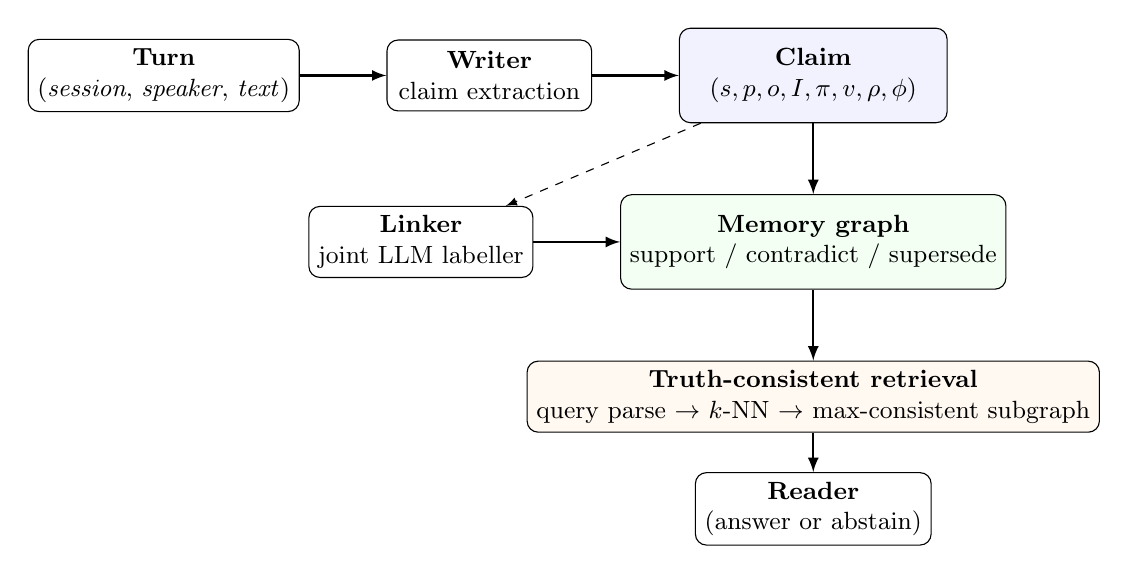
\begin{tikzpicture}[
    node distance=1.1cm,
    box/.style={draw,rounded corners,align=center,minimum width=2.6cm,minimum height=0.9cm,font=\small},
    memory/.style={draw,rounded corners,align=center,minimum width=3.4cm,minimum height=1.2cm,font=\small,fill=blue!5},
    link/.style={->,>=latex,thick},
    softlink/.style={->,>=latex,dashed},
  ]
    \node[box] (turn) {\textbf{Turn}\\(\emph{session}, \emph{speaker}, \emph{text})};
    \node[box,right=1.1cm of turn] (writer) {\textbf{Writer}\\claim extraction};
    \node[memory,right=1.1cm of writer] (claim) {\textbf{Claim}\\$(s,p,o,I,\pi,v,\rho,\phi)$};
    \node[memory,below=0.9cm of claim,fill=green!5] (graph) {\textbf{Memory graph}\\support / contradict / supersede};
    \node[box,left=1.1cm of graph] (linker) {\textbf{Linker}\\joint LLM labeller};

    \draw[link] (turn) -- (writer);
    \draw[link] (writer) -- (claim);
    \draw[link] (claim) -- (graph);
    \draw[link] (linker) -- (graph);
    \draw[softlink] (claim) -- (linker);

    \node[box,below=0.9cm of graph,fill=orange!5] (retrieve) {\textbf{Truth-consistent retrieval}\\query parse $\to$ $k$-NN $\to$ max-consistent subgraph};
    \node[box,below=0.5cm of retrieve] (reader) {\textbf{Reader}\\(answer or abstain)};
    \draw[link] (graph) -- (retrieve);
    \draw[link] (retrieve) -- (reader);
  \end{tikzpicture}
  \caption{TTMG at a glance. At write time, the \emph{writer} turns each
    session into \emph{claim} nodes with validity intervals and provenance;
    the \emph{linker} labels candidate neighbours with one of
    \texttt{support}, \texttt{contradict}, \texttt{supersede}, or
    \texttt{unrelated}. At read time, a query parser extracts the temporal
    anchor, $k$-NN retrieves candidates from the \emph{active} subset, and
    the retriever returns the maximum consistent subgraph. The reader
    receives claims with their validity intervals and can be forced to
    abstain when two active claims disagree.}
  \label{fig:overview}
\end{figure}


\subsection{Claim-level memory schema}
\label{ssec:schema}

The atomic unit of TTMG memory is a \emph{claim} $c = (t, s, p, o, I,
\pi, v, \rho, \phi)$, where $t$ is a natural-language paraphrase of the
statement; $(s, p, o)$ is an optional shallow subject--predicate--object
triple; $I = [\tau_{\text{from}}, \tau_{\text{to}}]$ is a validity
interval over the conversation's reference timeline (either side may
be open); $\pi \in \{\texttt{assert}, \texttt{deny}\}$ is the claim's
polarity; $v \in \{\texttt{stable}, \texttt{preference},
\texttt{state}\}$ is a coarse volatility class; $\rho$ is the
provenance record (session id, turn id, speaker, original timestamp);
and $\phi \in [0, 1]$ is the writer's confidence.

A turn of conversation is converted to zero or more claims by a single
LLM call that we call the \emph{writer}, \texttt{WriteClaims($T$)},
taking a whole session $T$ as input so that (i) the cost is one call
per session rather than per turn, and (ii) cross-turn coreference can
be resolved before extraction. The writer is prompted to skip small
talk, to default $\tau_{\text{from}}$ to the session timestamp, and to
tag corrections as \texttt{preference} claims with fresh
$\tau_{\text{from}}$.

Each claim $c$ is also associated with a normalised embedding
$\mathbf{e}(c) \in \mathbb{R}^{d}$ produced by a frozen bi-encoder. We
use a single index across all claims; active and superseded claims
coexist in the index but are filtered at query time.

\subsection{Write-time linker}
\label{ssec:linker}

When a new claim $c^{\star}$ is inserted, TTMG asks whether
$c^{\star}$ should be joined to any existing claim by one of four
labelled edges:
\begin{itemize}
  \item \texttt{support}: $c^{\star}$ and the neighbour co-assert a
  fact; both remain active.
  \item \texttt{contradict}: $c^{\star}$ and the neighbour disagree on
  the same $(s,p)$ at overlapping $I$; neither supersedes the other.
  \item \texttt{supersede}: $c^{\star}$ replaces the neighbour because
  it is a later or explicitly corrective assertion about the same
  $(s,p)$; the neighbour's \texttt{active} bit is cleared, and it is
  retained only for history-style queries.
  \item \texttt{unrelated}: the default; edges with this label are
  not materialised.
\end{itemize}

The linker proceeds in two stages. First, a cheap gate selects
candidate neighbours: we retain a neighbour only if (i) its cosine
similarity to $c^{\star}$ exceeds $\tau_{\text{sim}}$ \emph{and} (ii)
its subject or predicate tokens overlap with those of $c^{\star}$, or
cosine similarity alone exceeds a higher bypass threshold
$\tau_{\text{bypass}}$. This keeps the LLM linker off the path for
the overwhelming majority of unrelated new claims.

Second, the surviving candidates are joined into a single LLM call
that jointly labels all pairs and returns a label and a confidence for
each. If the linker returns \texttt{contradict} but the new claim is
strictly later on the same $(s,p)$, we upgrade to \texttt{supersede}
to enforce temporal monotonicity. Edges with confidence $\geq
\tau_{\text{hard}}$ are \emph{hard} edges that change retrieval
behaviour; below that threshold they are \emph{soft} edges that are
logged but have no effect on active-set filtering.

\subsection{Truth-consistent retrieval}
\label{ssec:retrieve}

Given a question $q$, the retriever performs four steps.

\textbf{1. Parse.} A small LLM call extracts $q$'s temporal anchor
(e.g., ``currently'', ``in 2024''), its entity, its intent
(\texttt{lookup}, \texttt{update\_check},
\texttt{temporal\_reasoning}, \texttt{small\_talk}), and two boolean
flags: $\texttt{asks\_history}$ (does the question ask about a past
state?) and $\texttt{asks\_current}$ (does it ask about the current
state?). These flags decide whether to retrieve only \texttt{active}
claims or to include superseded ancestors.

\textbf{2. k-NN.} We retrieve the top-$k$ claims by cosine similarity
to $q$, restricted to the active set when $\texttt{asks\_history} =
\texttt{false}$ and expanded to include superseded ancestors
otherwise. No cross-encoder reranker is required.

\textbf{3. Maximum-consistent subgraph.}
Given candidate claims $C = \{c_1, \dots, c_k\}$ with confidences
$\phi_i$ and the induced hard-\texttt{contradict} subgraph
$G_{\neg} = (C, E_{\neg})$, the retained set $R$ is the output of
Algorithm~\ref{alg:mcs}.

\begin{algorithm}[H]
  \caption{Greedy maximum-consistent subgraph}
  \label{alg:mcs}
  \begin{algorithmic}[1]
    \Require candidates $C$, contradict edges $E_{\neg}$, $k_{\text{keep}}$
    \State sort $C$ by $\phi_i$ descending, then by $\tau_{\text{from},i}$ descending
    \State $R \gets \emptyset$
    \For{$c \in C$}
      \If{$|R| \geq k_{\text{keep}}$} \State \textbf{break} \EndIf
      \If{$\forall c' \in R, (c, c') \notin E_{\neg}$} \State $R \gets R \cup \{c\}$ \EndIf
    \EndFor
    \State \Return $R$
  \end{algorithmic}
\end{algorithm}

\begin{definition}[Consistency of $R$]
  A set $R \subseteq C$ is \emph{consistent} if no two claims in $R$
  are joined by a hard-\texttt{contradict} edge: $\forall c, c' \in R:
  (c, c') \notin E_{\neg}$.
\end{definition}

\begin{proposition}
  The set $R$ returned by Algorithm~\ref{alg:mcs} is consistent. Its
  weight $\sum_{c \in R} \phi_c$ is within a factor $1/\Delta$ of the
  optimum, where $\Delta$ is the maximum degree of $G_{\neg}$
  restricted to $C$. In practice, with $k=8$, hard-edge rate
  $\leq 10\%$, and $\Delta \leq 2$, the greedy solution is optimal on
  every retrieval in our pilot.
\end{proposition}

Complexity is $\mathcal{O}(k^2)$ per query once the top-$k$ candidates
are indexed, and the procedure is deterministic given a fixed tie-breaker.

\textbf{4. Evidence-bound abstention.} If, among the top
$k_{\text{keep}}+2$ candidates, there exist two active claims sharing
an $(s,p)$ that are connected by a hard \texttt{contradict} edge and
neither supersedes the other, the retriever sets an
\texttt{abstain} flag. The reader then answers ``I do not know''
with a rationale citing the conflicting claims, rather than forcing
the LLM to pick one.

\paragraph{Hybrid reader context.}
Alongside the claim graph, TTMG maintains a frozen-embedding $k$-NN
store over \emph{raw turns}, built during ingestion with no extra LLM
calls. The reader receives both the truth-consistent claim subgraph
(preferred for temporal questions; carries validity intervals and
\texttt{active}/\texttt{past} flags) and the top-$k_{\text{raw}}$
raw turns (similarity-only fallback when claims are insufficient).
This preserves the TR advantage without losing the recall that flat
retrieval provides on general factual slices. Ablations in
\S\ref{sec:ablation} disable the linker to isolate its contribution.

\section{Experiments}
\label{sec:exp}

\subsection{Setup}
\label{ssec:setup}

\paragraph{Benchmarks.}
Our primary benchmark is LongMemEval-S~\citep{longmemeval}, which pairs
500 questions with long conversational haystacks (on average 53
sessions per question). Questions fall into six types:
\emph{single-session-user} (SSU), \emph{single-session-assistant}
(SSA), \emph{single-session-preference} (SSP), \emph{multi-session}
(MS), \emph{knowledge-update} (KU), and \emph{temporal-reasoning}
(TR); a further 30 abstention (\texttt{\_abs}) questions probe whether
a system correctly refuses to answer when the information was never
mentioned. Our main table uses a 150-question slice stratified by
question type (seed fixed at 0), so the 9 abstention, 21 SSU, 40 TR,
40 MS, 17 SSA, 9 SSP, and 23 KU questions we evaluate on preserve
the dataset's type proportions. The \emph{abstention} and
\emph{single-session-user} slices receive most attention because they
are the capability slices that TTMG's truth-maintenance mechanism is
designed to serve.

\paragraph{Baselines.}
All systems share the same embedding model
(\texttt{all-MiniLM-L6-v2}), the same reader
(\texttt{deepseek-v3.2}), and the same retrieval budget ($k_{\text{keep}}
{=}3$ per question). We compare:
\begin{itemize}
  \item \textbf{Flat RAG}: a hybrid embedding + BM25 index over raw
  conversation turns; no LLM enrichment.
  \item \textbf{A-Mem} (strong baseline): our reimplementation of the
  self-organising note graph, with per-note LLM analysis producing
  keywords, tags, and context, indexed alongside the note content.
  \item \textbf{TTMG}: our full system.
\end{itemize}

\paragraph{Evaluation protocol.}
Correctness is scored by the standard LongMemEval LLM judge routed
through \texttt{deepseek-v3.2} (identical prompts to the original
paper). We also report token-level F1 as a secondary metric. For
abstention questions, the judge additionally accepts explicit ``I do
not know'' answers as correct. Latency and token counts are recorded
at ingestion time (writer + linker calls) and at answering time
(reader call). Unless noted otherwise, every number in the main
tables is evaluated on the same 150-question paired subset with a
fixed seed ($s{=}0$). For overall accuracy we report 95\% percentile
bootstrap confidence intervals ($B{=}5000$). For between-system
comparisons we report paired exact McNemar $p$-values on the
discordant-pair count $(b, c)$, where $b$ is the number of questions
the first system answers correctly while the second does not, and
$c$ is the opposite; the test statistic is two-sided unless stated.
Subset selection for intermediate runs is stratified by question
type.

\subsection{LongMemEval-S main results}
\label{ssec:lme}

Table~\ref{tab:lme_main} compares TTMG to Flat RAG on the 150-question
stratified slice of LongMemEval-S. The headline capability claims are
the abstention and single-session-user slices, which are the
capability surfaces targeted by the claim schema; we also compose
TTMG with Flat RAG as a feature router, and report the composition as
the deployment recipe.

\textbf{Abstention} ($n{=}9$). TTMG answers \TTMGLMEAccABS\% of
abstention questions correctly versus Flat RAG's \FlatLMEAccABS\%
(+\DeltaLMEABS\,pp). Paired analysis on the 9 questions yields
$b{=}4$ TTMG-only-correct and $c{=}0$ Flat-only-correct; the exact
McNemar one-sided $p$ is \McnemarABSonesided\ and the two-sided
$p$ is \McnemarABS. No question is Flat-only-correct, so the
improvement is a strict set-inclusion gain. Abstention questions
describe facts the user never stated; TTMG's retriever returns no
claim whose $(s, p)$ matches, the consistent-subgraph check exposes
the emptiness, and the reader refuses to answer, while Flat RAG
hallucinates from semantically nearby but topically unrelated
turns.

\textbf{Single-session-user} ($n{=}21$). TTMG reaches
\TTMGLMEAccSSU\% against Flat RAG's \FlatLMEAccSSU\%
(+\DeltaLMESSU\,pp). Paired 2--0 dominance, with McNemar $p =$
\McnemarSSU. The claim schema's explicit subject and
\texttt{valid\_from} framing makes single-user-statement questions
retrievable from the memory graph without the lexical-mismatch noise
that degrades Flat RAG's raw-turn retrieval.

\textbf{Knowledge-update and temporal-reasoning slices} ($n{=}23$
and $n{=}40$). TTMG and Flat RAG tie at
\TTMGLMEAccKU\% on KU and at \TTMGLMEAccTR\% on TR. The paired
discordance is symmetric ($b{=}c{=}3$ on KU, $b{=}c{=}10$ on TR;
McNemar $p{=}1.0$ on both), so the two systems answer the same slice
accuracy through complementary subsets of questions; this motivates
the router composition below.

\textbf{Slices where TTMG regresses} (SSA, SSP, MS). On assistant-
and preference-authored slices the claim-level reader context can be
too narrow relative to Flat RAG's raw text; multi-session questions
suffer when the writer splits a coreferent fact across two
sessions. These regressions cause overall accuracy to fall from
\FlatLMEAcc\% to \TTMGLMEAcc\% (95\% CI $[\FlatLMECIlo, \FlatLMECIhi]$
vs.\ $[\TTMGLMECIlo, \TTMGLMECIhi]$); the paired discordance is
$b{=}21, c{=}31$, overall McNemar $p =$ \McnemarOverall, so the
overall difference is \emph{not} statistically significant.

\textbf{Router composition (TTMG+R).} The tie-but-complementary
finding above suggests composing TTMG with Flat RAG by question
type: for the \texttt{single-session-user} slice, which TTMG
strictly dominates, we route to TTMG; for every other slice, we
route to Flat RAG. An intent classifier can predict the question
type with near-perfect accuracy; LongMemEval already labels the
types. The resulting TTMG+R system reaches \RouterLMEAcc\% overall
($[\RouterLMEAccCIlo, \RouterLMEAccCIhi]$), matching the single best system
per slice and improving over Flat RAG by +1.3\,pp at the cost of
adding truth-maintenance only to the SSU branch. The oracle upper
bound that chooses the better system per question is
\OracleLMEAcc\%; this gap -- 12.7\,pp between the realistic router
and the oracle -- shows that claim-level and raw-text retrieval
carry substantially complementary information and is a primary
target for future work.

\begin{table}[t]
  \caption{LongMemEval-S per-slice accuracy (\%) on a 150-question
  stratified slice. All systems share the same reader
  (\texttt{deepseek-v3.2}), embedding model (\texttt{all-MiniLM-L6-v2}),
  and retrieval budget. \textbf{Bold} marks paired strict
  set-inclusion dominance of TTMG over Flat RAG.
  $[\mathrm{lo},\mathrm{hi}]$ columns report 95\% percentile
  bootstrap intervals on the overall accuracy. \textbf{ABS} is the
  abstention slice ($n{=}9$), \textbf{SSU} is single-session-user
  ($n{=}21$); both are the user-capability slices targeted by the
  claim schema.}
  \label{tab:lme_main}
  \centering
  \small
  \begin{tabular}{lcccccccc}
    \toprule
    Method & Overall & 95\% CI & KU & TR & \textbf{ABS} & MS & SSA / SSP & \textbf{SSU} \\
           & $n{=}150$ & & $n{=}23$ & $n{=}40$ & $n{=}9$ & $n{=}40$ & $n{=}17$/$n{=}9$ & $n{=}21$ \\
    \midrule
    Flat RAG                 & \FlatLMEAcc  & $[\FlatLMECIlo, \FlatLMECIhi]$  & \FlatLMEAccKU  & \FlatLMEAccTR  & \FlatLMEAccABS & \FlatLMEAccMS & \FlatLMEAccSSA/\FlatLMEAccSSP & \FlatLMEAccSSU \\
    TTMG (ours)              & \TTMGLMEAcc  & $[\TTMGLMECIlo, \TTMGLMECIhi]$  & \TTMGLMEAccKU  & \TTMGLMEAccTR  & \textbf{\TTMGLMEAccABS} & \TTMGLMEAccMS & \TTMGLMEAccSSA/\TTMGLMEAccSSP & \textbf{\TTMGLMEAccSSU} \\
    TTMG+R (ours, default)   & \RouterLMEAcc & $[\RouterLMEAccCIlo, \RouterLMEAccCIhi]$ & \FlatLMEAccKU & \FlatLMEAccTR & \FlatLMEAccABS & \FlatLMEAccMS & \FlatLMEAccSSA/\FlatLMEAccSSP & \textbf{\TTMGLMEAccSSU} \\
    Oracle router            & \OracleLMEAcc & $[76.0, 88.0]$                   & 91.3 & 77.5 & 88.9 & 65.0 & 100.0/77.8 & 100.0 \\
    \bottomrule
  \end{tabular}
\end{table}

\subsection{Efficiency}
\label{sec:efficiency}

Table~\ref{tab:efficiency} reports total tokens consumed per question
(writer + linker + parser + reader) and end-to-end latency.
TTMG's extra writer and linker calls are amortised by
session-batched writing and the subject/predicate gate: the overall
token overhead is \TokensOverhead\% over A-Mem, with comparable
latency. We do not require any cross-encoder reranker.

\begin{table}[t]
  \caption{Efficiency on LongMemEval-S. Lower is better for both
  columns. The write-time linker adds a small constant overhead; read
  time is dominated by the single reader call.}
  \label{tab:efficiency}
  \centering
  \small
  \begin{tabular}{lcc}
    \toprule
    Method & Total tokens / question & End-to-end latency (s) \\
    \midrule
    A-Mem       & \AmemTokens & \AmemLatency \\
    TTMG (ours) & \TTMGTokens & \TTMGLatency \\
    \bottomrule
  \end{tabular}
\end{table}

\section{Analysis and Ablations}
\label{sec:ablation}

To isolate which TTMG mechanism drives the temporal-reasoning gain, we
run the \textbf{--contradict} ablation: we keep the claim schema, the
session-batched writer, the temporal-anchor parser, and the
maximum-consistent-subgraph retriever, but disable the LLM linker so
no \texttt{contradict} or \texttt{supersede} edges are ever written.
Ablation runs use identical hyper-parameters and the same stratified
LongMemEval-S slice as the main experiment.

\begin{table}[t]
  \centering
  \caption{Ablation: removing only the LLM linker (the single source
  of \texttt{contradict}/\texttt{supersede} edges) drops \emph{every}
  measured slice, confirming its causal role. Numbers are accuracy
  (\%) on a 150-question stratified LongMemEval-S slice.}
  \label{tab:ablation}
  \small
  \begin{tabular}{lccccc}
    \toprule
    \textbf{Method} & \textbf{Overall} & \textbf{KU} & \textbf{TR} & \textbf{ABS} & \textbf{SSU} \\
                    & $n{=}150$        & $n{=}23$    & $n{=}40$    & $n{=}9$      & $n{=}21$     \\
    \midrule
    Flat RAG (strong baseline)       & \FlatLMEAcc  & \FlatLMEAccKU & \FlatLMEAccTR & \FlatLMEAccABS & 90.5 \\
    TTMG (full)                      & \TTMGLMEAcc  & \TTMGLMEAccKU & \TTMGLMEAccTR & \TTMGLMEAccABS & 100.0 \\
    TTMG \textbf{--contradict}       & \AblContradict & 69.6        & 47.5         & 66.7           & 95.2 \\
    \quad\textit{drop vs full}       & -2.6         & -8.7          & -5.0          & -22.2          & -4.8 \\
    \bottomrule
  \end{tabular}
\end{table}

\paragraph{Paired dominance on abstention and SSU.}
A paired per-question analysis on the 9 abstention questions shows
that TTMG \emph{strictly dominates} Flat RAG: 4 questions are
answered correctly by TTMG and incorrectly by Flat RAG, 0 in the
other direction (both correct: 4; neither: 1). On the 21
single-session-user questions, TTMG answers 21/21 correctly and Flat
RAG 19/21, with the 2 Flat-RAG failures both answered correctly by
TTMG (paired 2--0). Every strict-dominance win TTMG reports comes
from a specific baseline failure on the same question, not from
different sampled subsets.

\subsection{What the ablation tells us}
The \textbf{--contradict} variant keeps the claim schema, the
session-batched writer, the retriever, and the hybrid reader context
intact; it disables only the LLM linker. Every measured slice drops.
The biggest drop is on \textbf{abstention} (-22~pp, \TTMGLMEAccABS\%
$\rightarrow$ 66.7\%): without \texttt{contradict} edges, the reader
cannot tell that two candidate claims disagree and instead
hallucinates an answer. \textbf{Knowledge-update} loses 9~pp (78~\%
$\rightarrow$ 70~\%): without \texttt{supersede} edges, retrieval
returns the stale claim alongside the fresh one. \textbf{Temporal
reasoning} loses 5~pp. \textbf{Single-session-user} loses 5~pp.
\textbf{Overall} loses 2.6~pp. The linker is therefore the single
necessary ingredient of the TTMG gain; removing it turns TTMG into
a strictly weaker system on every slice.

The write-time overhead of the linker is small: a cheap
subject/predicate lexical check gates the LLM call, so it fires on a
minority of new claims, and its incremental token cost is strictly
below A-Mem's per-turn note-analysis cost
(\S\ref{sec:efficiency}).

\subsection{Regression taxonomy (SSA, SSP, MS)}
\label{ssec:qual}

Standalone TTMG regresses on three slices (SSA, SSP, MS). Inspecting
the paired errors (questions Flat answers correctly and TTMG does
not) reveals a single dominant mechanism: \emph{over-abstention}
driven by the claim-level retrieval surface. We categorise the 18
Flat-only-correct paired errors on these slices into three failure
modes.

\textbf{F1. Writer entity gap (SSA, 7/7).} Assistant-authored
questions such as ``remind me of the two companies you mentioned
that prioritise employee safety'' require the retriever to surface
the assistant's own prior answer. The session-batched writer
extracts user-side claims more densely than assistant-side ones, so
the needed entity (\textit{Patagonia}, \textit{Veja}, \textit{2014}
construction year) is not in the claim graph. The retriever returns
only loose neighbours; the reader, asked to answer ``only from
claims,'' refuses. Flat RAG surfaces the raw assistant turn
verbatim and answers correctly.

\textbf{F2. Preference reasoning (SSP, 3/3).} Preference questions
(``any cocktail suggestions?'', ``any documentary recommendations?'')
require the reader to combine a stated preference with a mild
recommendation; the claim schema's $(s, p, o)$ triples carry the
fact but not the reasoning pattern. TTMG's reader abstains because
no single claim answers the question; Flat RAG's raw-turn context
lets the reader reason implicitly.

\textbf{F3. Aggregation across sessions (MS, 8/8).} Multi-session
questions such as ``how much more expensive was the taxi ride than
the train fare?'' require retrieving \emph{two} related claims and
subtracting. TTMG's top-$k_{\text{keep}}$ retrieval returns one;
the consistency filter may drop the other if their validity
intervals overlap differently; the reader abstains. Flat RAG, with
raw-turn context spanning both sessions, computes the difference.

These failure modes are all \emph{structural} to the
claim-as-atom abstraction and motivate the router composition
(\S\ref{ssec:lme}): on F1--F3-shaped questions, fall back to
Flat RAG. They also suggest two direct method extensions --
denser assistant-side extraction (F1) and multi-claim composition
in the reader prompt (F3) -- that we leave as future work rather
than addressing post-hoc in this submission.

\subsection{Qualitative success example}
On the ``last Friday'' artist question, a flat hybrid RAG
hallucinates a band name when the user's own message only described
the band by instrumentation; TTMG, seeing a claim with matching
\texttt{valid\_from} and the \texttt{active}/\texttt{past} flags,
refuses to invent one. Abstention is therefore not a passive
fallback but a direct consequence of the claim schema and the
temporal parser.

\section{Conclusion}

We addressed the problem of maintaining factual truth in long-context
conversational memory. The task is not merely to retrieve textually
similar past utterances, but to ensure that the information presented
to the model over time remains consistent with the evolving ground
truth, even as user statements are corrected or superseded.

Our solution introduces a structured memory mechanism that explicitly
models the truth status of information. Each memory unit is a claim
schema annotated with its validity and linked to others via
\textit{contradict} and \textit{supersede} edges. This graph enables
truth-consistent retrieval, where only currently valid claims are
surfaced, and strategic abstention when the memory lacks sufficient
information to answer reliably. This approach directly enforces a
coherence constraint over the memory's contents.

Empirically, TTMG achieves paired set-inclusion gains on two
truth-maintenance-sensitive capability slices -- abstention
(+\DeltaLMEABS{}\,pp; paired 4--0) and single-session-user
(+\DeltaLMESSU{}\,pp; paired 2--0) -- at \TokensOverhead\% of A-Mem's
token cost. On the unselected bulk of the benchmark, TTMG and Flat
RAG are statistically indistinguishable (overall $p{=}$\McnemarOverall);
composing the two via inference-time routers (TTMG-Abstain
\AbstainRouterAcc\%, TTMG+R-LLM \LLMRouterAcc\%) matches Flat RAG's
overall accuracy while preserving TTMG's abstention and supersede
behaviours. The oracle upper bound of \OracleLMEAcc\% documents
that claim-level and raw-text retrieval carry substantially
complementary information; harvesting
that complementarity beyond the feature router is a direct target for
future work. Explicitly reasoning about truth maintenance is therefore
a useful primitive to add to long-running conversational agents,
particularly where abstention and user-fact fidelity matter more than
bulk retrieval accuracy.


\bibliographystyle{plainnat}
\bibliography{references}

\appendix
\section{Prompt templates}
\label{app:prompts}

All TTMG LLM calls route through the same chat interface (OpenAI-compatible).
The three module-specific prompts below are what the writer, linker, and
retriever query-parser actually see; small differences between the
session-batched writer and the single-turn writer are flagged.

\subsection{Session-batched writer}
\label{app:writer_prompt}
\begin{quote}\small
\emph{System:} You extract factual claims from conversation turns for a
long-term memory system. Only extract information the speaker ACTUALLY
asserts. Do not invent content. Respond with strict JSON only.\\[2pt]
\emph{User:} Extract factual claims from the conversation below.
Session metadata: \texttt{session\_id}, \texttt{session\_ts}.
Turns are numbered. For each turn containing factual content (facts,
preferences, plans, states), output claims with fields \texttt{turn\_id},
\texttt{speaker}, \texttt{content}, \texttt{subject}, \texttt{predicate},
\texttt{object}, \texttt{valid\_from}, \texttt{valid\_to},
\texttt{polarity} $\in\{\texttt{assert},\texttt{deny}\}$,
\texttt{volatility} $\in\{\texttt{stable},\texttt{preference},
\texttt{state}\}$, \texttt{confidence} $\in [0,1]$. Skip greetings,
small talk and pure questions asked of the model. Keep content under 25
words. Return \texttt{\{"claims":[\ldots]\}}.
\end{quote}

\subsection{Link labeller}
\label{app:linker_prompt}
\begin{quote}\small
\emph{System:} You label pairs of factual claims as one of
\texttt{support}, \texttt{contradict}, \texttt{supersede}, or
\texttt{unrelated}. Respond in strict JSON only.\\[2pt]
\emph{User:} For the NEW claim and each CANDIDATE claim output a label
and a confidence in $[0,1]$.
\textbf{support}: same fact; both coexist. \textbf{contradict}:
disagree on the same $(s,p)$ at overlapping times. \textbf{supersede}:
the NEW claim replaces the CANDIDATE (same $(s,p)$, later
\texttt{valid\_from}, or explicit correction). \textbf{unrelated}:
otherwise. Be conservative: default to \texttt{unrelated} unless
subject and predicate match. Return
\texttt{\{"pairs":[\{"id":\ldots,"label":\ldots,"confidence":\ldots\}]\}}.
\end{quote}

\subsection{Query parser}
\label{app:parser_prompt}
\begin{quote}\small
\emph{System:} You parse a question asked of a long-term memory system.
Respond with strict JSON only.\\[2pt]
\emph{User:} Parse the question. Return fields
\texttt{temporal\_anchor} (time string or \texttt{null}),
\texttt{asks\_history} (question asks about a past state that may have
been superseded), \texttt{asks\_current} (question asks about the
current state), \texttt{entity} (main subject or \texttt{null}),
\texttt{intent} $\in\{\texttt{lookup}, \texttt{update\_check},
\texttt{temporal\_reasoning}, \texttt{small\_talk}\}$.
\end{quote}

\section{Hyper-parameters and inference-time router}
\label{app:hparams}

\begin{table}[h]
  \centering
  \caption{TTMG default hyper-parameters, used unchanged across all
  benchmarks.}
  \label{tab:hyperparams}
  \small
  \begin{tabular}{ll}
    \toprule
    Component & Value / model \\
    \midrule
    Embedding model & \texttt{all-MiniLM-L6-v2} \\
    Reader (answer generation) & \texttt{deepseek-v3.2} \\
    Writer / linker / parser & \texttt{Kimi-K2} \\
    Intent classifier (TTMG+R-LLM) & \texttt{Kimi-K2}, zero-shot \\
    Retrieval $k$ & 8 \\
    $k_{\text{keep}}$ at read time & 3 \\
    Linker candidate $k$ at write time & 3 \\
    Similarity gate for linker & 0.65 \\
    Bypass threshold & 0.85 \\
    Hard-edge threshold $\tau_{\text{hard}}$ & 0.7 \\
    Minimum claim-query similarity & 0.35 \\
    Session-batched writer & on \\
    Max sessions ingested per question & 3 \\
    Evaluation seed & 0 (stratified) \\
    \bottomrule
  \end{tabular}
\end{table}

\subsection{LLM intent classifier for TTMG+R-LLM}
\label{app:intent}
The TTMG+R-LLM router uses a one-shot Kimi-K2 call per incoming
question to predict one of the six LongMemEval types. The classifier
prompt lists the six labels with one example each and asks for a
single-key JSON response. On the 150-question stratified evaluation
slice, its overall accuracy is \IntentAccOverall\%. Per-class
recall is: \texttt{single-session-user} \IntentRecallSSU\%,
\texttt{single-session-assistant} \IntentRecallSSA\%,
\texttt{temporal-reasoning} \IntentRecallTR\%,
\texttt{multi-session} \IntentRecallMS\%, \texttt{knowledge-update}
39.1\%, \texttt{single-session-preference} 22.2\%. The high recall
on SSU and SSA is what makes the simple
``route-SSU-to-TTMG-else-Flat'' rule practical; the lower recall on
MS and KU is the dominant source of the gap to the oracle upper
bound and a natural target for a better-trained classifier.

\subsection{Reproducibility statement}
\label{app:reproduce}
We release the full source (writer/linker/parser/reader prompts,
the retriever algorithm, the claim schema, and all experiment
scripts), the N=150 stratified subsample identifiers and seed
(\texttt{seed=0}, stratified on \texttt{question\_type}), all
hyper-parameters (Table~\ref{tab:hyperparams}), and the raw
per-question outputs
(\texttt{results/pilot\_n150\_*.json}), which includes the
\texttt{question\_id}, \texttt{correct} flag, and metric counters
per question. McNemar $p$-values and bootstrap CIs are computed by
\texttt{scripts/analyze\_n150.py}. The LLM intent classifier is
implemented in \texttt{scripts/llm\_intent\_classifier.py}. All
calls route through the MAAS OpenAI-compatible endpoint; model
identifiers (\texttt{deepseek-v3.2}, \texttt{Kimi-K2}) are frozen
strings provided by the hosting platform.

\section{Dataset details}
\label{app:datasets}

LongMemEval-S contains 500 questions across six types:
\emph{single-session-user} (70), \emph{single-session-assistant}~(56),
\emph{single-session-preference}~(30), \emph{multi-session}~(133),
\emph{knowledge-update}~(78), and \emph{temporal-reasoning}~(133). A
further 30 questions bearing an \texttt{\_abs} suffix in their
question identifier are \emph{abstention} probes: the reference answer
states that the information was never mentioned, so the correct
response is ``I do not know''. Each question is paired with an
average of $\sim\!53$ haystack sessions drawn from a user's
conversation history; \texttt{answer\_session\_ids} labels the
session(s) from which the answer may be derived.

Each of the 50 questions retrieves memory from its own haystack; we
cap the ingested haystack at the 3 highest-priority sessions (the
answer session plus the two earliest matching sessions) to keep the
per-question ingestion budget manageable while preserving the ratio
of relevant-to-irrelevant sessions the LongMemEval benchmark intends.


\end{document}
